%!TEX root = ../thesis.tex
\section{製程參數因子描述}
\label{c:ch4.1}
在染色製程中許多的因子會影響染後之染色表現因子,如染劑濃度、助劑濃度、初始pH值、浴比值、主泵浦速率、帶布輪速率、升溫速率、持溫溫度、水洗時間、皂洗升溫速率、皂洗持溫溫度、皂洗時間等。本研究計畫先聚焦於實驗室所能控制之製程參數:浴比值、升溫速率、持溫溫度、水洗時間、皂洗升溫速率、皂洗持溫溫度、皂洗時間等。染色製程參數與染色表現因子關聯分析,首先以統計實驗設計方法釐清關鍵之製程因子,並分析染色製程參數與染色表現因子關聯。但由於要得到各染色表現因子間的關係性必須透過實驗的方式,且也需考量實驗的成本,所以本研究由染整工廠建議及文獻當中,先針對特定幾項製程參數進行實驗。
\begin{figure} 
\centering  

\includegraphics[width=12cm,height=8cm]{Graph/graph3.png}
\caption{聚酯纖維布料在染整階段時間與溫度關係}
\label{fig:graph3}
\end{figure}
圖\ref{fig:graph3}為第一階段染色製程,可以知道染色在升溫時,當溫度從常溫$T_0$到達$T_1$後就必須讓升溫速率降低,持續到升溫為$T_2$時在提升升溫速率。由於布料的性質,如果在染液升溫區間升溫太快,容易造成布料吸收不均的情況發生,因此在紡織業界也稱此區間為”危險區間“,經過此區間後。布料材質為聚酯纖維下必須要分三個階段來進行升溫,在圖\ref{fig:graph3}中為常溫,因為不同磅數的匹布在最高溫的設定會對染布吸收顏色能力上有一定的影響,所以及為我們設定的溫度參數。至於$\alpha$則為第二階段升溫時的升溫速率,由於$\alpha$的設定也會影響其他的製程參數,所以$\alpha$也納入我們設定的參數。而t為染布浸泡在染液中的持溫時間,時間越長吸收越好越穩定,但同時也會占用機台的產能,造成成本上升,故持溫時間也需列入考慮。最後由於升溫的速率及持溫的時間長短都會受到浴比值的影響,當浴比值越大則所需消耗的燃料成本就會相對較多,因此我們根據上列五個主要影響成本的因子做實驗設計,藉此來描繪各因子間與染色表現間的反應關係。

我們藉由分析以及與業者討論後,找出各因子間與染色表現因子或是成本間的反應關係。但由於在實驗室中,我們只能藉由檢測儀器檢測相關的染色表現因子,如色差值($\Delta E$)或固色力($K/S$),本研究計畫擬推估每次實驗所設定之製程參數,其相對應的染整過程所需耗用能源及水的總成本,如圖3.2
\begin{figure} 
\centering  
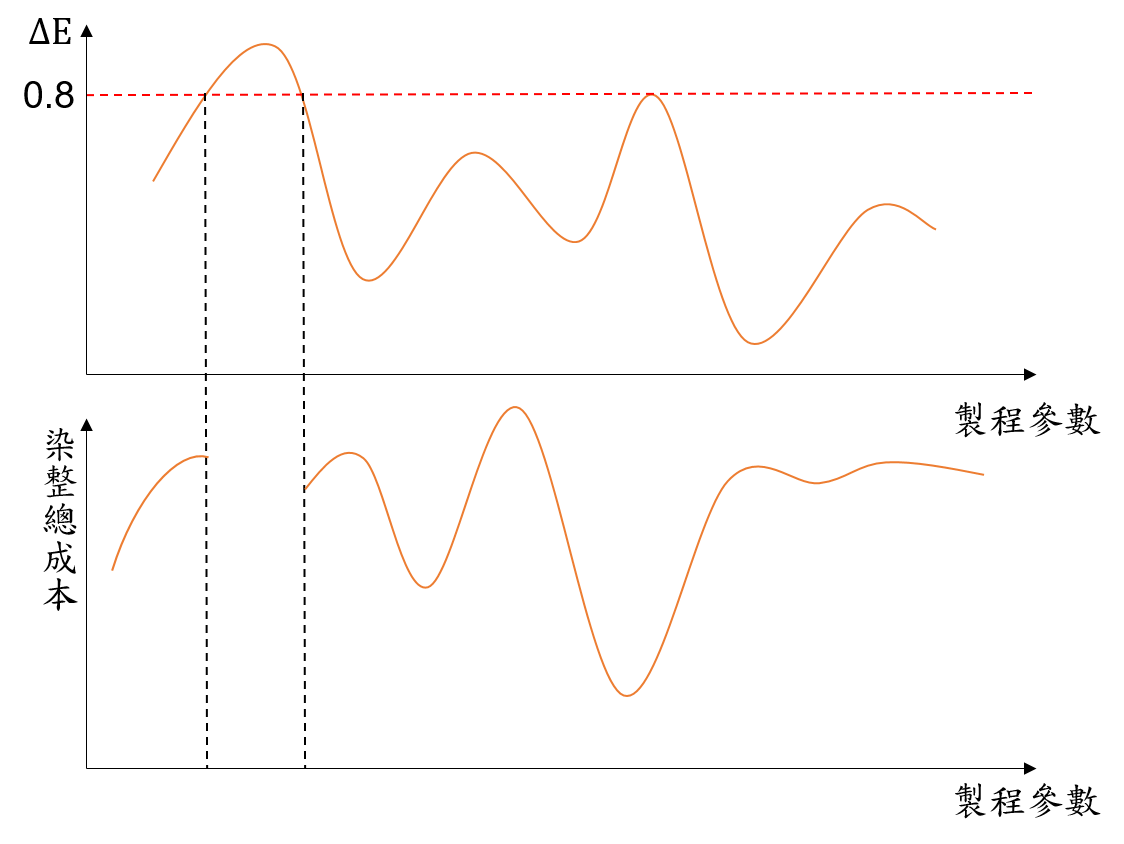
\includegraphics[width=12cm,height=10cm]{Graph/graph4.png}
\caption{聚染整總成本與色差值間的關係}
\label{fig:graph4}
\end{figure}

圖~\ref{fig:graph4}為成本與色差值間的關係示意圖,在圖~\ref{fig:graph4}的上半部為在固定染色配方下,描述各製程參數與色差值間的關係,從對應的製程參數設定,可推估染整廠實際所需花費的操作成本。而圖~\ref{fig:graph4}下半部則為染整製程總成本與製程參數間的關係。由圖~\ref{fig:graph4}可知下半部總成本有部分的區塊被截掉,原因是該製程參數所對應的色差值已經超出所規定的色差,故該區塊的製程總成本不列入成本的模型內。在本研究中由染色製程參數與染色表現因子關聯分析,能夠先分析出製程參數及色差值間的反應曲面,而在對應模型中,製程參數及總成本間的模型能夠互相對應,便能成功從色差值轉換為成本模型。

染色製程參數優化技術,以染色製程參數與染色表現因子關聯分析為輸入資訊,建構染色製程參數優化模型,描述上述製程因子對生產成本及品質成本之影響,搜尋製程總成本最低的製程參數組合。但由於「染色製程參數與染色表現因子關聯分析」需要分析各因子間的組合,就必須針對實際情況得到相對應的實驗數據,在實際染整工廠內進行實驗,對染整工廠來說成本是相當高,所以在「染色製程參數與染色表現因子關聯分析」中,只能從實驗室以5公克的布料來實驗。但從實驗結果得知相對的反應曲面,無法實際描繪出染整現場可能面對的製程參數變異,而造成品質成本的增加。再者,由於實驗室所做的實驗只能以5公克的布料來實驗,布的單次使用量非常的少,因此當製程參數在實驗室找出最佳製程參數結果,轉移到現場工廠內大量的布及大量的染料使用時,便可能會出現與實驗不同的結果。

在生產過程中除了考慮減少生產成本外,我們還需要考慮生產變異所造成的品質成本。在本研究中我們為了總成本最低的情況下符合品質外,我們還分別對品質成本搜尋最佳化結果,作為使用者調整生產以及品質間的平衡的依據,因此本研究將主要分成三個模型來表示第一個模型為生產成本模型(運作成本模型),第二個模型為品質穩健度模型,最後一個模型為品質模型($\Delta E$模型)。
